\documentclass[12pt]{article}\usepackage[]{graphicx}\usepackage[]{color}
%% maxwidth is the original width if it is less than linewidth
%% otherwise use linewidth (to make sure the graphics do not exceed the margin)
\makeatletter
\def\maxwidth{ %
  \ifdim\Gin@nat@width>\linewidth
    \linewidth
  \else
    \Gin@nat@width
  \fi
}
\makeatother

\definecolor{fgcolor}{rgb}{0.345, 0.345, 0.345}
\newcommand{\hlnum}[1]{\textcolor[rgb]{0.686,0.059,0.569}{#1}}%
\newcommand{\hlstr}[1]{\textcolor[rgb]{0.192,0.494,0.8}{#1}}%
\newcommand{\hlcom}[1]{\textcolor[rgb]{0.678,0.584,0.686}{\textit{#1}}}%
\newcommand{\hlopt}[1]{\textcolor[rgb]{0,0,0}{#1}}%
\newcommand{\hlstd}[1]{\textcolor[rgb]{0.345,0.345,0.345}{#1}}%
\newcommand{\hlkwa}[1]{\textcolor[rgb]{0.161,0.373,0.58}{\textbf{#1}}}%
\newcommand{\hlkwb}[1]{\textcolor[rgb]{0.69,0.353,0.396}{#1}}%
\newcommand{\hlkwc}[1]{\textcolor[rgb]{0.333,0.667,0.333}{#1}}%
\newcommand{\hlkwd}[1]{\textcolor[rgb]{0.737,0.353,0.396}{\textbf{#1}}}%

\usepackage{framed}
\makeatletter
\newenvironment{kframe}{%
 \def\at@end@of@kframe{}%
 \ifinner\ifhmode%
  \def\at@end@of@kframe{\end{minipage}}%
  \begin{minipage}{\columnwidth}%
 \fi\fi%
 \def\FrameCommand##1{\hskip\@totalleftmargin \hskip-\fboxsep
 \colorbox{shadecolor}{##1}\hskip-\fboxsep
     % There is no \\@totalrightmargin, so:
     \hskip-\linewidth \hskip-\@totalleftmargin \hskip\columnwidth}%
 \MakeFramed {\advance\hsize-\width
   \@totalleftmargin\z@ \linewidth\hsize
   \@setminipage}}%
 {\par\unskip\endMakeFramed%
 \at@end@of@kframe}
\makeatother

\definecolor{shadecolor}{rgb}{.97, .97, .97}
\definecolor{messagecolor}{rgb}{0, 0, 0}
\definecolor{warningcolor}{rgb}{1, 0, 1}
\definecolor{errorcolor}{rgb}{1, 0, 0}
\newenvironment{knitrout}{}{} % an empty environment to be redefined in TeX

\usepackage{alltt}
%\VignetteEngine{knitr::knitr}

\usepackage[hidelinks, breaklinks=true]{hyperref}
\usepackage{natbib}
\usepackage{longtable}
\usepackage{multirow}
\usepackage{rotating}
\usepackage{bm}
\usepackage{booktabs}
\usepackage[table]{xcolor}
%\usepackage{ulem}
\usepackage[utf8]{inputenc}
\usepackage{geometry}


\title{Supporting information for \\
\textbf{Analysis of statistical interactions in factorial experiments}}
\author{Andreas Kitsche, Frank Schaarschmidt}
\IfFileExists{upquote.sty}{\usepackage{upquote}}{}
\begin{document}
%\VignetteIndexEntry{Using statint package} 
%\VignettePackage{statint} \\


\maketitle

\begin{abstract}
This manuscript provides some supporting information to the article \textbf{Analysis of statistical interactions in factorial experiments} \citep{Kitsche.2014}.
It presents the application of the \verb@iacontrast()@ and \verb@plotcontrast()@ function in the \verb@statint@ package to generate a labelled product type interaction contrast matrix for a detailed analysis of statistical interactions in the two-way layout. Furthermore, the analysis of statistical interactions of some selected data sets from the agronomy and crop sciences are demonstrated in case studies. 
\end{abstract}
\tableofcontents

\newpage
The package \verb@statint()@ is currently uploaded at \url{https://github.com/AKitsche/statint}.
To install directly from github, the package \verb@devtools@ is needed (available on CRAN):
\begin{knitrout}
\definecolor{shadecolor}{rgb}{0.969, 0.969, 0.969}\color{fgcolor}\begin{kframe}
\begin{alltt}
\hlkwd{install.packages}\hlstd{(}\hlstr{"devtools"}\hlstd{)}
\hlkwd{library}\hlstd{(devtools)}
\hlkwd{install_github}\hlstd{(}\hlkwc{username} \hlstd{=} \hlstr{"AKitsche"}\hlstd{,} \hlkwc{repo} \hlstd{=} \hlstr{"statint"}\hlstd{)}
\hlkwd{library}\hlstd{(statint)}
\end{alltt}
\end{kframe}
\end{knitrout}



\section{Usage of iacontrast() function}
The function \verb@iacontrast()@ generates a labelled interaction contrast matrix for the anaylsis of statistical interactions in two-way layouts. The user has to commit the two factor variables \verb@fa@ and \verb@fb@ and the types of the two one-way contrasts \verb@typea@ and \verb@typeb@. Alternatively, the user can apply a-priori defined one-way contrast matrices \verb@cma@ and \verb@cmb@.

The output is a list with two elements: i) \verb@fab@ a new factor generated by all pair-wise combinations of the levels of the two factors from the two-way layout, ii)\verb@cmab@ a labelled interaction contrast matrix.


In the following the interaction contrast matrix is generated using the Dunnett type contrast (comparisons to a control) for the first factor and the Tukey type contrast (all pair-wise comparisons) for the second factor in a 4-by-3 layout.
\begin{knitrout}
\definecolor{shadecolor}{rgb}{0.969, 0.969, 0.969}\color{fgcolor}\begin{kframe}
\begin{alltt}
\hlcom{# generating factor variables}
\hlstd{fa} \hlkwb{<-} \hlkwd{factor}\hlstd{(}\hlkwd{rep}\hlstd{(}\hlkwd{rep}\hlstd{(LETTERS[}\hlnum{1}\hlopt{:}\hlnum{4}\hlstd{],} \hlkwd{rep}\hlstd{(}\hlnum{3}\hlstd{,} \hlnum{4}\hlstd{)),} \hlkwc{each} \hlstd{=} \hlnum{3}\hlstd{))}
\hlstd{fb} \hlkwb{<-} \hlkwd{factor}\hlstd{(}\hlkwd{rep}\hlstd{(}\hlkwd{rep}\hlstd{(}\hlkwd{c}\hlstd{(}\hlnum{1}\hlstd{,} \hlnum{2}\hlstd{,} \hlnum{3}\hlstd{),} \hlkwd{rep}\hlstd{(}\hlnum{3}\hlstd{,} \hlnum{3}\hlstd{)),} \hlkwc{times} \hlstd{=} \hlnum{4}\hlstd{))}
\hlkwd{library}\hlstd{(statint)}
\hlkwd{iacontrast}\hlstd{(}\hlkwc{fa} \hlstd{= fa,} \hlkwc{fb} \hlstd{= fb,} \hlkwc{typea} \hlstd{=} \hlstr{"Dunnett"}\hlstd{,} \hlkwc{typeb} \hlstd{=} \hlstr{"Tukey"}\hlstd{)}
\end{alltt}
\end{kframe}
\end{knitrout}

% latex table generated in R 3.0.2 by xtable 1.7-1 package
% Mon Mar 24 09:14:16 2014
\begin{table}[ht]
\centering
{\scriptsize
\begin{tabular}{rrrrrrrrrrrrr}
  \hline
 & A:1 & A:2 & A:3 & B:1 & B:2 & B:3 & C:1 & C:2 & C:3 & D:1 & D:2 & D:3 \\ 
  \hline
((B - A):2) - ((B - A):1) & 1 & -1 & 0 & -1 & 1 & 0 & 0 & 0 & 0 & 0 & 0 & 0 \\ 
  ((B - A):3) - ((B - A):1) & 1 & 0 & -1 & -1 & 0 & 1 & 0 & 0 & 0 & 0 & 0 & 0 \\ 
  ((B - A):3) - ((B - A):2) & 0 & 1 & -1 & 0 & -1 & 1 & 0 & 0 & 0 & 0 & 0 & 0 \\ 
  ((C - A):2) - ((C - A):1) & 1 & -1 & 0 & 0 & 0 & 0 & -1 & 1 & 0 & 0 & 0 & 0 \\ 
  ((C - A):3) - ((C - A):1) & 1 & 0 & -1 & 0 & 0 & 0 & -1 & 0 & 1 & 0 & 0 & 0 \\ 
  ((C - A):3) - ((C - A):2) & 0 & 1 & -1 & 0 & 0 & 0 & 0 & -1 & 1 & 0 & 0 & 0 \\ 
  ((D - A):2) - ((D - A):1) & 1 & -1 & 0 & 0 & 0 & 0 & 0 & 0 & 0 & -1 & 1 & 0 \\ 
  ((D - A):3) - ((D - A):1) & 1 & 0 & -1 & 0 & 0 & 0 & 0 & 0 & 0 & -1 & 0 & 1 \\ 
  ((D - A):3) - ((D - A):2) & 0 & 1 & -1 & 0 & 0 & 0 & 0 & 0 & 0 & 0 & -1 & 1 \\ 
   \hline
\end{tabular}
}
\end{table}



The function \verb@plotcontrast()@ plots a contrast matrix in a tile plane with rectangles. It requires a contrast matrix in which the rownames represent the names for the comparisons of interest and the colnames represent the levels of the factor of interest. Contrast coefficients with a negative sign are displayed in red, whereas contrast coefficients with a positive are displayed in blue. 

\begin{knitrout}
\definecolor{shadecolor}{rgb}{0.969, 0.969, 0.969}\color{fgcolor}\begin{kframe}
\begin{alltt}
\hlstd{IntContrastMat} \hlkwb{<-} \hlkwd{iacontrast}\hlstd{(}\hlkwc{fa} \hlstd{= fa,} \hlkwc{fb} \hlstd{= fb,} \hlkwc{typea} \hlstd{=} \hlstr{"Dunnett"}\hlstd{,} \hlkwc{typeb} \hlstd{=} \hlstr{"Tukey"}\hlstd{)}
\hlkwd{plotcontrast}\hlstd{(IntContrastMat}\hlopt{$}\hlstd{cmab)}
\end{alltt}
\end{kframe}
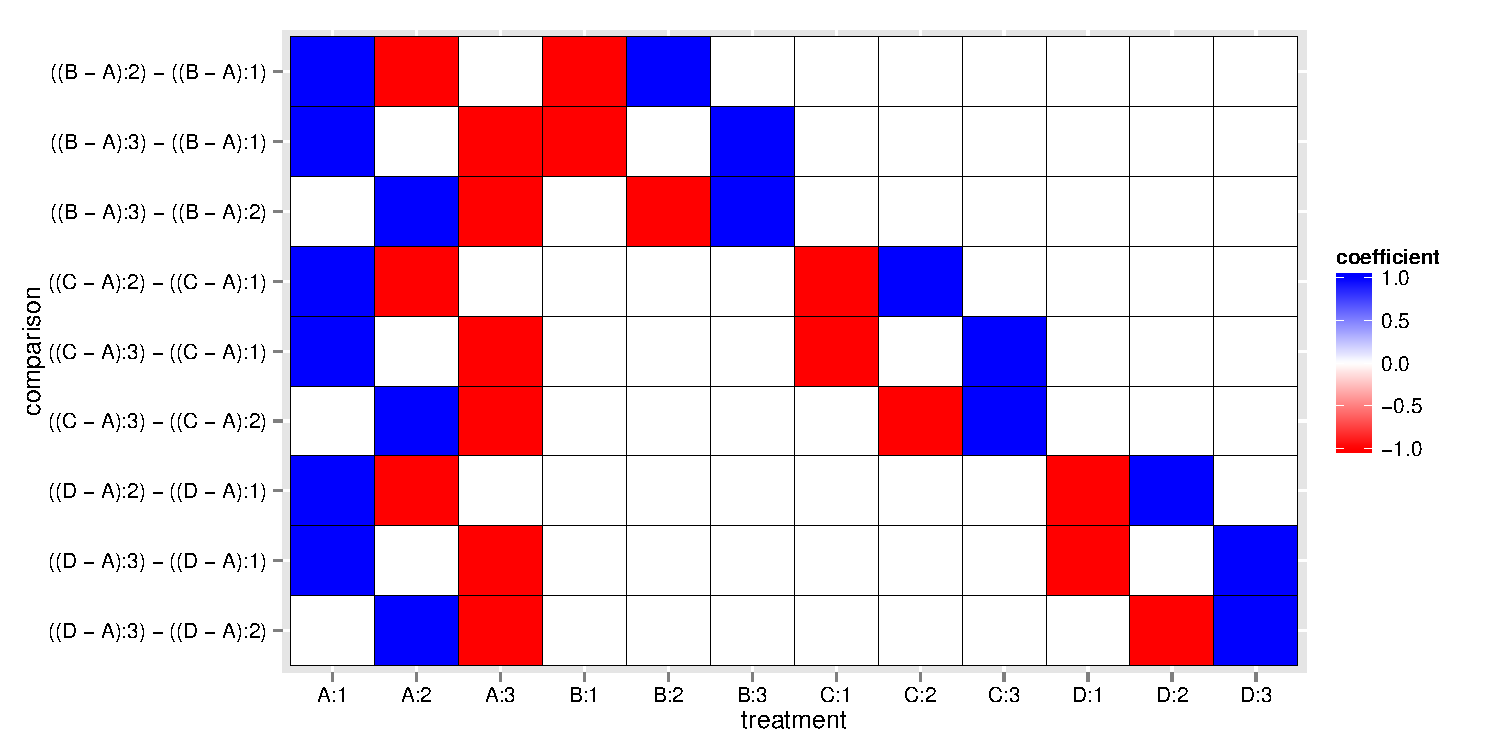
\includegraphics[width=\maxwidth]{figure/chunk12b} 

\end{knitrout}



We next demonstrate the usage of prespecified user defined contrasts.
\begin{knitrout}
\definecolor{shadecolor}{rgb}{0.969, 0.969, 0.969}\color{fgcolor}\begin{kframe}
\begin{alltt}
\hlcom{#generating user defined one-way contrast matrices}
\hlstd{ContrastsA} \hlkwb{<-} \hlkwd{matrix}\hlstd{(}\hlkwd{c}\hlstd{(}\hlnum{1} \hlstd{,} \hlnum{1}\hlstd{,} \hlopt{-}\hlnum{1}\hlstd{,} \hlopt{-}\hlnum{1}\hlstd{,}
                       \hlnum{1} \hlstd{,}\hlopt{-}\hlnum{1}\hlstd{,}  \hlnum{0}\hlstd{,}  \hlnum{0}\hlstd{,}
                       \hlnum{0} \hlstd{,} \hlnum{0}\hlstd{,}  \hlnum{1}\hlstd{,} \hlopt{-}\hlnum{1}\hlstd{),} \hlkwc{nrow}\hlstd{=}\hlnum{3}\hlstd{,} \hlkwc{byrow}\hlstd{=}\hlnum{TRUE}\hlstd{)}
\hlstd{ContrastsB} \hlkwb{<-} \hlkwd{matrix}\hlstd{(}\hlkwd{c}\hlstd{(}\hlopt{-}\hlnum{1}\hlstd{,} \hlnum{0.5}\hlstd{,} \hlnum{0.5}\hlstd{,}
                        \hlnum{0}\hlstd{,}   \hlnum{1}\hlstd{,}  \hlopt{-}\hlnum{1}\hlstd{),} \hlkwc{nrow}\hlstd{=}\hlnum{2}\hlstd{,} \hlkwc{byrow}\hlstd{=}\hlnum{TRUE}\hlstd{)}
\hlkwd{iacontrast}\hlstd{(}\hlkwc{fa}\hlstd{=fa,} \hlkwc{fb}\hlstd{=fb,} \hlkwc{cma}\hlstd{=ContrastsA,} \hlkwc{cmb}\hlstd{=ContrastsB)}
\end{alltt}
\end{kframe}
\end{knitrout}


\tiny
% latex table generated in R 3.0.2 by xtable 1.7-1 package
% Mon Mar 24 09:14:16 2014
\begin{table}[ht]
\centering
{\scriptsize
\begin{tabular}{rrrrrrrrrrrrr}
  \hline
 & A:1 & A:2 & A:3 & B:1 & B:2 & B:3 & C:1 & C:2 & C:3 & D:1 & D:2 & D:3 \\ 
  \hline
((A,B - C,D):2,3) - ((A,B - C,D):1) & -1.0 & 0.5 & 0.5 & -1.0 & 0.5 & 0.5 & 1.0 & -0.5 & -0.5 & 1.0 & -0.5 & -0.5 \\ 
  ((A,B - C,D):2) - ((A,B - C,D):3) & 0.0 & 1.0 & -1.0 & 0.0 & 1.0 & -1.0 & 0.0 & -1.0 & 1.0 & 0.0 & -1.0 & 1.0 \\ 
  ((A - B):2,3) - ((A - B):1) & -1.0 & 0.5 & 0.5 & 1.0 & -0.5 & -0.5 & 0.0 & 0.0 & 0.0 & 0.0 & 0.0 & 0.0 \\ 
  ((A - B):2) - ((A - B):3) & 0.0 & 1.0 & -1.0 & 0.0 & -1.0 & 1.0 & 0.0 & 0.0 & 0.0 & 0.0 & 0.0 & 0.0 \\ 
  ((C - D):2,3) - ((C - D):1) & 0.0 & 0.0 & 0.0 & 0.0 & 0.0 & 0.0 & -1.0 & 0.5 & 0.5 & 1.0 & -0.5 & -0.5 \\ 
  ((C - D):2) - ((C - D):3) & 0.0 & 0.0 & 0.0 & 0.0 & 0.0 & 0.0 & 0.0 & 1.0 & -1.0 & 0.0 & -1.0 & 1.0 \\ 
   \hline
\end{tabular}
}
\end{table}


\normalsize

\begin{knitrout}
\definecolor{shadecolor}{rgb}{0.969, 0.969, 0.969}\color{fgcolor}\begin{kframe}
\begin{alltt}
\hlstd{IntContrastMat} \hlkwb{<-} \hlkwd{iacontrast}\hlstd{(}\hlkwc{fa} \hlstd{= fa,} \hlkwc{fb} \hlstd{= fb,} \hlkwc{cma} \hlstd{= ContrastsA,} \hlkwc{cmb} \hlstd{= ContrastsB)}
\hlkwd{plotcontrast}\hlstd{(IntContrastMat}\hlopt{$}\hlstd{cmab)}
\end{alltt}
\end{kframe}
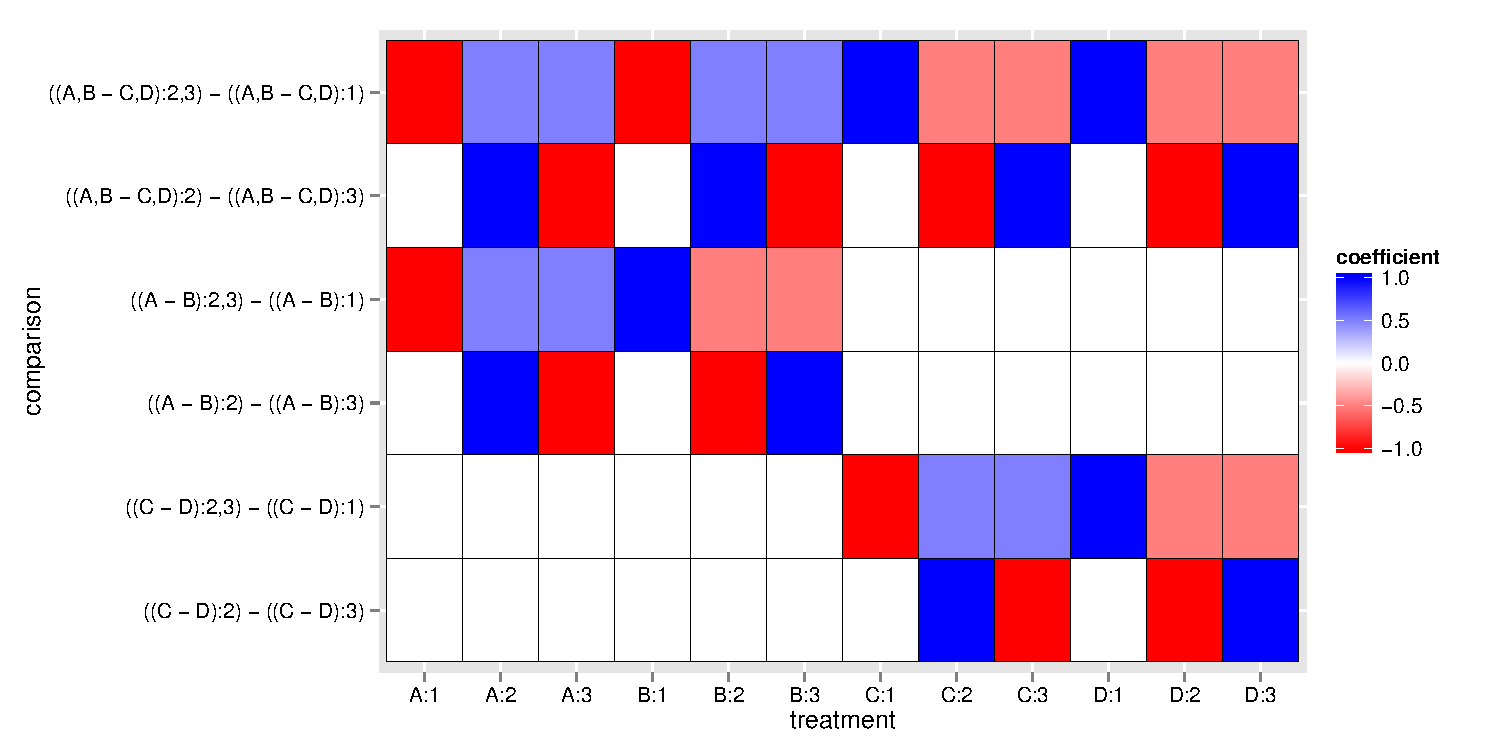
\includegraphics[width=\maxwidth]{figure/chunk14b} 

\end{knitrout}


\newpage
\section{Lettuce data set}
The \verb@lettuce@ data set presents a simulated data set, inspired by the example presented in \cite{Bradu.1974}. The example is an experiment conducted to analyse the effects of soil type and phosphate
fertilizers on lettuce crops. The primary response variable was dry matter measured in grams per plot.
Three different soil types, namely S1, S2 and S3, and four different levels of phosphate fertilization
(including an untreated control) were investigated in a balanced, completely cross-classified treatment
structure, laid out as completely randomized design with four replications per treatment combination.

\begin{knitrout}
\definecolor{shadecolor}{rgb}{0.969, 0.969, 0.969}\color{fgcolor}\begin{kframe}
\begin{alltt}
\hlkwd{data}\hlstd{(lettuce)}
\hlkwd{str}\hlstd{(lettuce)}
\hlcom{#reorder Fertilizer levels}
\hlstd{lettuce}\hlopt{$}\hlstd{Fertilizer} \hlkwb{<-} \hlkwd{factor}\hlstd{(lettuce}\hlopt{$}\hlstd{Fertilizer,}
        \hlkwc{levels}\hlstd{=}\hlkwd{c}\hlstd{(}\hlstr{"control"}\hlstd{,}\hlstr{"cal.phos"}\hlstd{,} \hlstr{"magn.phos"}\hlstd{,}\hlstr{"pot.metaphos"}\hlstd{))}
\end{alltt}
\end{kframe}
\end{knitrout}


\begin{knitrout}
\definecolor{shadecolor}{rgb}{0.969, 0.969, 0.969}\color{fgcolor}\begin{figure}[]

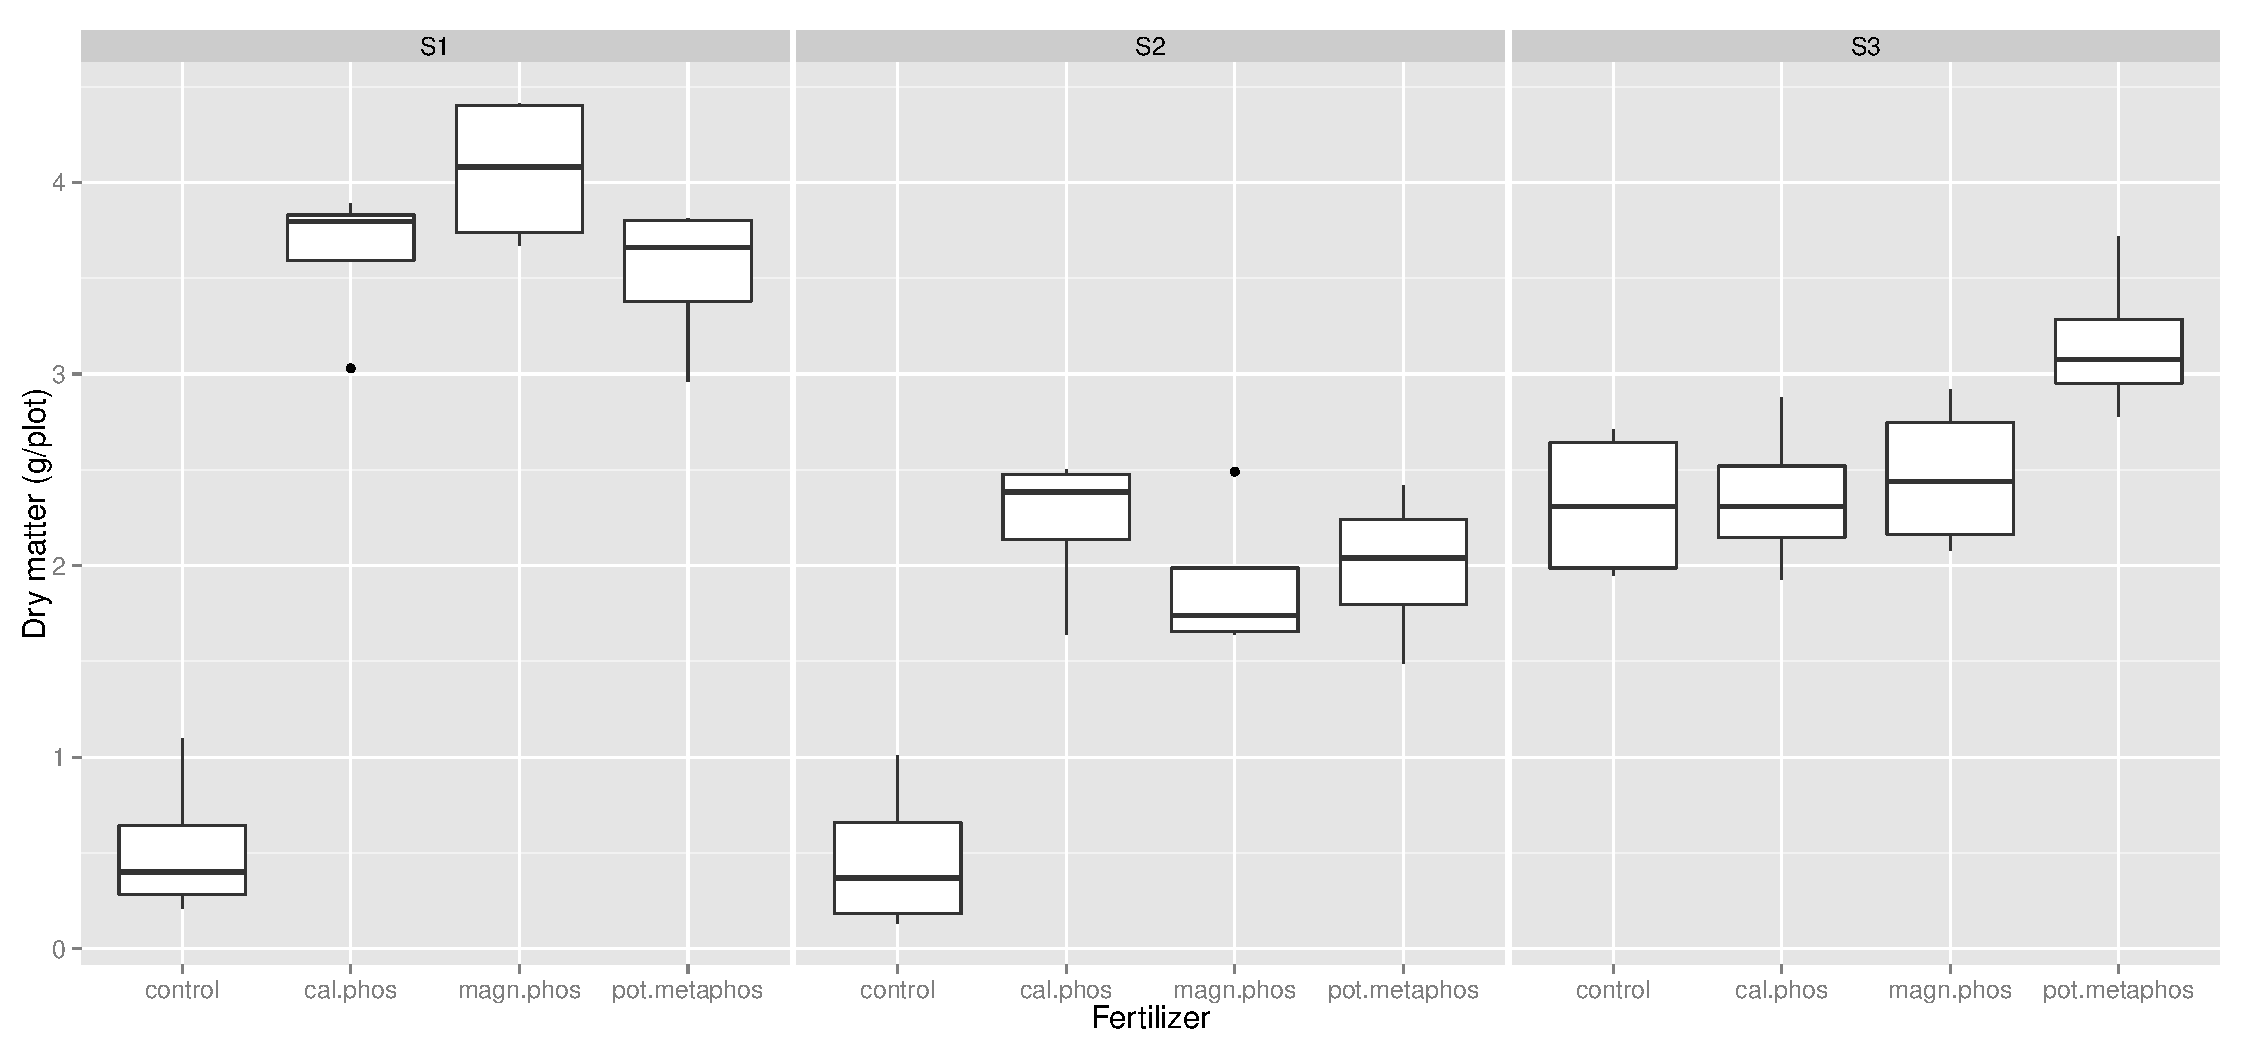
\includegraphics[width=\maxwidth]{figure/chunk32} \caption[Boxplots of the dry matter based on each fertilizer-by-soil type combination]{Boxplots of the dry matter based on each fertilizer-by-soil type combination.\label{fig:chunk32}}
\end{figure}


\end{knitrout}


The factor fertilizer consists of
an untreated control group and three different phosphorus fertilizers. The objective of including this factor is to
estimate the increase in yield that results applying each of the fertilizers compared to the untreated
control. The second factor, soil type, contains no
further substructure, and interest is in comparing all three soil types among each other. The product type interaction contrasts allow to
interpret to what extend the difference in yield between the three phosphate fertilizers compared to
the control varies between the three soil types.

% latex table generated in R 3.0.2 by xtable 1.7-1 package
% Mon Mar 24 09:14:17 2014
\begin{table}[ht]
\centering
\begin{tabular}{lrrrrr}
  \hline
 & Df & Sum Sq & Mean Sq & F value & Pr($>$F) \\ 
  \hline
Fertilizer & 3 & 26.41 & 8.80 & 55.00 & 0.0000 \\ 
  Soil & 2 & 14.08 & 7.04 & 43.98 & 0.0000 \\ 
  Fertilizer:Soil & 6 & 14.65 & 2.44 & 15.25 & 0.0000 \\ 
  Residuals & 36 & 5.76 & 0.16 &  &  \\ 
   \hline
\end{tabular}
\caption{Two-way ANOVA of the Lettuce data set.} 
\end{table}



The interaction contrasts compare the differences
of the fertilizer effects between the soil types, where the fertilizer effects of interest are restricted
to the differences of each phosphorus fertilizer to the control group. 
To test the corresponding hypothesis fomulated by the interaction contrasts the function \verb@glht()@ in the package \verb@multcomp@ \citep{Hothorn.2008} is used. The corresponding multiplicity adjusted p-values and simutaneous confidence intervals are  available using the functions \verb@summary()@ and \verb@confint()@.

\begin{knitrout}
\definecolor{shadecolor}{rgb}{0.969, 0.969, 0.969}\color{fgcolor}\begin{kframe}
\begin{alltt}
\hlcom{#define appropriate user defined contrast matrices }
\hlstd{SoilMatrix} \hlkwb{<-} \hlkwd{matrix}\hlstd{(}\hlkwd{c}\hlstd{(}\hlnum{1}\hlstd{,} \hlopt{-}\hlnum{1}\hlstd{,} \hlnum{0}\hlstd{,}
                       \hlnum{1}\hlstd{,}  \hlnum{0}\hlstd{,}\hlopt{-}\hlnum{1}\hlstd{,}
                       \hlnum{0}\hlstd{,}  \hlnum{1}\hlstd{,}\hlopt{-}\hlnum{1}\hlstd{),} \hlkwc{nrow}\hlstd{=}\hlnum{3}\hlstd{,} \hlkwc{byrow}\hlstd{=}\hlnum{TRUE}\hlstd{)}
\hlstd{FertMatrix} \hlkwb{<-} \hlkwd{matrix}\hlstd{(}\hlkwd{c}\hlstd{(}\hlnum{1}\hlstd{,} \hlopt{-}\hlnum{1}\hlstd{,} \hlnum{0}\hlstd{,} \hlnum{0}\hlstd{,}
                       \hlnum{1}\hlstd{,}  \hlnum{0}\hlstd{,}\hlopt{-}\hlnum{1}\hlstd{,} \hlnum{0}\hlstd{,}
                       \hlnum{1}\hlstd{,}  \hlnum{0}\hlstd{,} \hlnum{0}\hlstd{,}\hlopt{-}\hlnum{1}\hlstd{),}\hlkwc{nrow}\hlstd{=}\hlnum{3}\hlstd{,} \hlkwc{byrow}\hlstd{=}\hlnum{TRUE}\hlstd{)}
\hlstd{InteractionContrasts} \hlkwb{<-} \hlkwd{iacontrast}\hlstd{(}\hlkwc{fa}\hlstd{=lettuce}\hlopt{$}\hlstd{Fertilizer,}
                                   \hlkwc{fb}\hlstd{=lettuce}\hlopt{$}\hlstd{Soil,}
                                   \hlkwc{cma}\hlstd{=FertMatrix,}
                                   \hlkwc{cmb}\hlstd{=SoilMatrix)}
\hlcom{#assign the pseudo one-way factor (Fertilizer-by-Soil) to the data set}
\hlstd{lettuce}\hlopt{$}\hlstd{FertSoil} \hlkwb{<-} \hlstd{InteractionContrasts}\hlopt{$}\hlstd{fab}
\hlcom{#fitting a cell means model using the pseudo one-way layout}
\hlstd{CMM} \hlkwb{<-} \hlkwd{lm}\hlstd{(Weight} \hlopt{~} \hlstd{FertSoil} \hlopt{-}\hlnum{1}\hlstd{,} \hlkwc{data} \hlstd{= lettuce)}
\hlcom{#Multiple Comparisons}
\hlstd{MultTest} \hlkwb{<-} \hlkwd{glht}\hlstd{(}\hlkwc{model}\hlstd{=CMM,}
                 \hlkwc{linfct} \hlstd{=} \hlkwd{mcp}\hlstd{(}\hlkwc{FertSoil}\hlstd{=InteractionContrasts}\hlopt{$}\hlstd{cmab))}
\hlkwd{summary}\hlstd{(MultTest)}\hlcom{#calculating adjusted p-values}
\hlkwd{confint}\hlstd{(MultTest)}\hlcom{#calculating simultaneous confidence intervals}
\end{alltt}
\end{kframe}
\end{knitrout}


% latex table generated in R 3.0.2 by xtable 1.7-1 package
% Mon Mar 24 09:14:18 2014
\begin{table}[ht]
\centering
{\scriptsize
\begin{tabular}{rrrrr}
  \hline
 & Estimate & Std.Error & t value & Pr($>$$|$t$|$) \\ 
  \hline
((control - cal.phos):S1) - ((control - cal.phos):S2) & -1.34 & 0.40 & -3.36 & 0.01 \\ 
  ((control - cal.phos):S1) - ((control - cal.phos):S3) & -3.06 & 0.40 & -7.65 & 0.00 \\ 
  ((control - cal.phos):S2) - ((control - cal.phos):S3) & -1.72 & 0.40 & -4.30 & 0.00 \\ 
  ((control - magn.phos):S1) - ((control - magn.phos):S2) & -2.10 & 0.40 & -5.25 & 0.00 \\ 
  ((control - magn.phos):S1) - ((control - magn.phos):S3) & -3.38 & 0.40 & -8.45 & 0.00 \\ 
  ((control - magn.phos):S2) - ((control - magn.phos):S3) & -1.28 & 0.40 & -3.21 & 0.02 \\ 
  ((control - pot.metaphos):S1) - ((control - pot.metaphos):S2) & -1.47 & 0.40 & -3.67 & 0.01 \\ 
  ((control - pot.metaphos):S1) - ((control - pot.metaphos):S3) & -2.15 & 0.40 & -5.38 & 0.00 \\ 
  ((control - pot.metaphos):S2) - ((control - pot.metaphos):S3) & -0.69 & 0.40 & -1.71 & 0.45 \\ 
   \hline
\end{tabular}
}
\caption{Results for the lettuce data set analysed with user defined interaction contrasts. Estimate denote the estimate for the comparison of interest, the adjusted P-value, Lower and Upper the lower and upper bound of the two-sided 0.95 simultaneous confidence interval.} 
\end{table}







\newpage
\section{Bush beans data set}
This example was published in \citet[p. 154]{Petersen.1985}. The data used within the \verb@statint@ package are simulated according to those in \cite{Petersen.1985}. A detailed description of the data set is given in \cite{Petersen.1985} and \cite{Kitsche.2014}.

We first analyse the data using a two-way ANOVA while including the block effect as fixed effect.




\begin{knitrout}
\definecolor{shadecolor}{rgb}{0.969, 0.969, 0.969}\color{fgcolor}\begin{kframe}
\begin{alltt}
\hlcom{# fitting a linear model and calculate an ANOVA}
\hlkwd{anova}\hlstd{(}\hlkwd{lm}\hlstd{(Yield} \hlopt{~} \hlstd{Variety} \hlopt{*} \hlstd{Spacing} \hlopt{+} \hlstd{Block,} \hlkwc{data} \hlstd{= beans))}
\end{alltt}
\end{kframe}
\end{knitrout}


% latex table generated in R 3.0.2 by xtable 1.7-1 package
% Mon Mar 24 09:14:18 2014
\begin{table}[ht]
\centering
\begin{tabular}{lrrrrr}
  \hline
 & Df & Sum Sq & Mean Sq & F value & Pr($>$F) \\ 
  \hline
Variety & 3 & 1332.56 & 444.19 & 34.22 & 0.0000 \\ 
  Spacing & 2 & 72.67 & 36.33 & 2.80 & 0.0754 \\ 
  Block & 3 & 341.90 & 113.97 & 8.78 & 0.0002 \\ 
  Variety:Spacing & 6 & 871.00 & 145.17 & 11.18 & 0.0000 \\ 
  Residuals & 33 & 428.35 & 12.98 &  &  \\ 
   \hline
\end{tabular}
\caption{Two-way ANOVA table of the bush beans data set} 
\end{table}




\cite{Kitsche.2014} described an alternative ANOVA that is also meaningful for this example, where the hierarchical structure between the growth type and the varieties within the growth type is taken into account. The resulting three-factorial ANOVA is given below.


\begin{knitrout}
\definecolor{shadecolor}{rgb}{0.969, 0.969, 0.969}\color{fgcolor}\begin{kframe}
\begin{alltt}
\hlstd{beans}\hlopt{$}\hlstd{Type[beans}\hlopt{$}\hlstd{Variety} \hlopt{==} \hlstr{"LittleGem"} \hlopt{|} \hlstd{beans}\hlopt{$}\hlstd{Variety}  \hlopt{==} \hlstr{"RedLake"}\hlstd{]} \hlkwb{<-} \hlstr{"erect"}
\hlstd{beans}\hlopt{$}\hlstd{Type[beans}\hlopt{$}\hlstd{Variety} \hlopt{==} \hlstr{"BigGreen"}  \hlopt{|} \hlstd{beans}\hlopt{$}\hlstd{Variety}  \hlopt{==} \hlstr{"NewEra"} \hlstd{]} \hlkwb{<-} \hlstr{"bushy"}
\hlkwd{anova}\hlstd{(}\hlkwd{lm}\hlstd{(Yield} \hlopt{~} \hlstd{Block} \hlopt{+}
                 \hlstd{Type} \hlopt{+}
                 \hlstd{Spacing} \hlopt{+}
                 \hlstd{Type}\hlopt{:}\hlstd{Spacing} \hlopt{+}
                 \hlstd{Type}\hlopt{:}\hlstd{Variety} \hlopt{+}
                 \hlstd{Type}\hlopt{:}\hlstd{Variety}\hlopt{:}\hlstd{Spacing,} \hlkwc{data}\hlstd{=beans))}
\end{alltt}
\end{kframe}
\end{knitrout}


% latex table generated in R 3.0.2 by xtable 1.7-1 package
% Mon Mar 24 09:14:18 2014
\begin{table}[ht]
\centering
\begin{tabular}{lrrrrr}
  \hline
 & Df & Sum Sq & Mean Sq & F value & Pr($>$F) \\ 
  \hline
Block & 3 & 341.90 & 113.97 & 8.78 & 0.0002 \\ 
  Type & 1 & 105.02 & 105.02 & 8.09 & 0.0076 \\ 
  Spacing & 2 & 72.67 & 36.33 & 2.80 & 0.0754 \\ 
  Type:Spacing & 2 & 748.17 & 374.08 & 28.82 & 0.0000 \\ 
  Type:Variety & 2 & 1227.54 & 613.77 & 47.28 & 0.0000 \\ 
  Type:Spacing:Variety & 4 & 122.83 & 30.71 & 2.37 & 0.0730 \\ 
  Residuals & 33 & 428.35 & 12.98 &  &  \\ 
   \hline
\end{tabular}
\caption{ANOVA table of the bush beans data set that takes the hierarchical structure between the growth type and the varieties within the growth type into account.} 
\end{table}


Fore a detailed analysis of the variety-by-spacing interaction we generate the appropriate one-way contrasts according to Table 9 and 10 in \cite{Kitsche.2014}. Afterwards, the corresponding product-type interaction contrast matrix (see Table 11 in \cite{Kitsche.2014}) is generated using the \verb@iacontrast()@ function.

\begin{knitrout}
\definecolor{shadecolor}{rgb}{0.969, 0.969, 0.969}\color{fgcolor}\begin{kframe}
\begin{alltt}
\hlstd{VarMat}   \hlkwb{<-} \hlkwd{matrix}\hlstd{(}\hlkwd{c}\hlstd{(}\hlnum{0.5}\hlstd{,}  \hlnum{0.5}\hlstd{,} \hlopt{-}\hlnum{0.5}\hlstd{,} \hlopt{-}\hlnum{0.5}\hlstd{,}
                       \hlnum{1}\hlstd{,}   \hlopt{-}\hlnum{1}\hlstd{,}    \hlnum{0}\hlstd{,}    \hlnum{0}\hlstd{,}
                       \hlnum{0}\hlstd{,}    \hlnum{0}\hlstd{,}    \hlnum{1}\hlstd{,}   \hlopt{-}\hlnum{1}\hlstd{),} \hlkwc{nrow}\hlstd{=}\hlnum{3}\hlstd{,} \hlkwc{byrow}\hlstd{=}\hlnum{TRUE}\hlstd{)}
\hlstd{SpaceMat} \hlkwb{<-} \hlkwd{matrix}\hlstd{(}\hlkwd{c}\hlstd{(}\hlnum{1}\hlstd{,} \hlopt{-}\hlnum{1}\hlstd{,}  \hlnum{0}\hlstd{,}
                     \hlnum{1}\hlstd{,}  \hlnum{0}\hlstd{,} \hlopt{-}\hlnum{1}\hlstd{,}
                     \hlnum{0}\hlstd{,}  \hlnum{1}\hlstd{,} \hlopt{-}\hlnum{1}\hlstd{),} \hlkwc{nrow}\hlstd{=}\hlnum{3}\hlstd{,} \hlkwc{byrow}\hlstd{=}\hlnum{TRUE}\hlstd{)}
\hlstd{InteractionMat} \hlkwb{<-} \hlkwd{iacontrast}\hlstd{(}\hlkwc{fa}\hlstd{=beans}\hlopt{$}\hlstd{Variety,} \hlkwc{fb}\hlstd{=beans}\hlopt{$}\hlstd{Spacing,}
                              \hlkwc{cma}\hlstd{=VarMat,} \hlkwc{cmb}\hlstd{=SpaceMat)}
\end{alltt}
\end{kframe}
\end{knitrout}

The hypotheses formulated in terms of the generated interaction contrasts are further tested using the \verb@glht()@ function in the package \verb@multcomp@ \citep{Hothorn.2008}. The corresponding multiplicity adjusted p-values and simutaneous confidence intervals are  available using the functions \verb@summary()@ and \verb@confint()@.
\begin{knitrout}
\definecolor{shadecolor}{rgb}{0.969, 0.969, 0.969}\color{fgcolor}\begin{kframe}
\begin{alltt}
\hlcom{#generating a new factor for the cell means}
\hlstd{beans}\hlopt{$}\hlstd{VarSpace} \hlkwb{<-} \hlstd{InteractionMat}\hlopt{$}\hlstd{fab}
\hlcom{#fitting a cell means model with the new factor}
\hlstd{CMM} \hlkwb{<-} \hlkwd{lm}\hlstd{(Yield} \hlopt{~} \hlstd{VarSpace} \hlopt{+} \hlstd{Block} \hlopt{-}\hlnum{1}\hlstd{,} \hlkwc{data} \hlstd{= beans)}
\hlcom{#Multiple Comparisons}
\hlkwd{library}\hlstd{(multcomp)}
\hlstd{MultTest} \hlkwb{<-} \hlkwd{glht}\hlstd{(}\hlkwc{model}\hlstd{=CMM,}
                 \hlkwc{linfct} \hlstd{=} \hlkwd{mcp}\hlstd{(}\hlkwc{VarSpace}\hlstd{=InteractionMat}\hlopt{$}\hlstd{cmab))}
\hlkwd{summary}\hlstd{(MultTest)}\hlcom{#calculating adjusted p-values}
\hlkwd{confint}\hlstd{(MultTest)}\hlcom{#calculating simultaneous confidence intervals}
\end{alltt}
\end{kframe}
\end{knitrout}





As an alternative analysis of the spacing-by-variety interaction the spacing factor could also be suggested as quantitative. In this case the comparison among regression slopes between varieties can be set up. Again it is assumed that interest is in the comparisons of the regression slopes between the different growth types and in comparisons of the varieties within the different growth types. 

For illustrative purposes we fit a linear mixed model assuming the Block as random factor. This results in a parameter vector of the fixed effects with four (variety specific) intercepts and four slopes. 
\begin{knitrout}
\definecolor{shadecolor}{rgb}{0.969, 0.969, 0.969}\color{fgcolor}\begin{kframe}
\begin{alltt}
\hlkwd{data}\hlstd{(beans)}
\hlkwd{str}\hlstd{(beans)}
\hlstd{beans}\hlopt{$}\hlstd{Variety} \hlkwb{<-}\hlkwd{factor}\hlstd{(beans}\hlopt{$}\hlstd{Variety,} \hlkwc{levels}\hlstd{=}\hlkwd{c}\hlstd{(}\hlstr{"BigGreen"}\hlstd{,}
                                               \hlstr{"NewEra"}\hlstd{,}
                                               \hlstr{"LittleGem"}\hlstd{,}
                                               \hlstr{"RedLake"}\hlstd{))}
\hlstd{beans}\hlopt{$}\hlstd{Spacing} \hlkwb{<-} \hlkwd{as.numeric}\hlstd{(beans}\hlopt{$}\hlstd{Spacing)}
\hlkwd{library}\hlstd{(nlme)}
\hlstd{fm1} \hlkwb{<-} \hlkwd{lme}\hlstd{(Yield} \hlopt{~} \hlstd{Variety}\hlopt{+}\hlstd{Variety}\hlopt{:}\hlstd{Spacing}\hlopt{-}\hlnum{1}\hlstd{,} \hlkwc{data}\hlstd{=beans,}
                                              \hlkwc{random}\hlstd{=} \hlopt{~} \hlnum{1}\hlopt{|}\hlstd{Block)}
\hlcom{#Generating user defined contrasts for the comparisons of the}
\hlcom{#regression slopes from the eight dimensional parameter vector}
\hlstd{Contrasts_Slopes} \hlkwb{<-} \hlkwd{matrix}\hlstd{(}\hlkwd{c}\hlstd{(}\hlnum{0} \hlstd{,} \hlnum{0}\hlstd{,} \hlnum{0}\hlstd{,} \hlnum{0}\hlstd{,} \hlnum{0.5}\hlstd{,} \hlnum{0.5}\hlstd{,}\hlopt{-}\hlnum{0.5}\hlstd{,}\hlopt{-}\hlnum{0.5}\hlstd{,}
                             \hlnum{0} \hlstd{,} \hlnum{0}\hlstd{,} \hlnum{0}\hlstd{,} \hlnum{0}\hlstd{,} \hlnum{1}  \hlstd{,}  \hlopt{-}\hlnum{1}\hlstd{,}   \hlnum{0}\hlstd{,}   \hlnum{0}\hlstd{,}
                             \hlnum{0} \hlstd{,} \hlnum{0}\hlstd{,} \hlnum{0}\hlstd{,} \hlnum{0}\hlstd{,} \hlnum{0}  \hlstd{,}   \hlnum{0}\hlstd{,}   \hlnum{1}\hlstd{,}  \hlopt{-}\hlnum{1}\hlstd{),}
                           \hlkwc{byrow}\hlstd{=}\hlnum{TRUE}\hlstd{,}
                           \hlkwc{nrow}\hlstd{=}\hlnum{3}\hlstd{)}
\hlkwd{row.names}\hlstd{(Contrasts_Slopes)} \hlkwb{<-} \hlkwd{c}\hlstd{(}\hlstr{"Bushy-Tall"}\hlstd{,}
                                 \hlstr{"Big Green-New Era"}\hlstd{,}
                                 \hlstr{"Little Gem-Red Lake"}\hlstd{)}
\hlcom{#testing the user defined comparisons of regression slopes}
\hlcom{#using the glht() function}
\hlstd{MultTest} \hlkwb{<-} \hlkwd{glht}\hlstd{(fm1,} \hlkwc{linfct} \hlstd{= Contrasts_Slopes)}
\hlkwd{summary}\hlstd{(MultTest)}
\end{alltt}
\end{kframe}
\end{knitrout}


% latex table generated in R 3.0.2 by xtable 1.7-1 package
% Mon Mar 24 09:14:19 2014
\begin{table}[ht]
\centering
{\normalsize
\begin{tabular}{rrrrr}
  \hline
 & Estimate & Std.Error & t value & Pr($>$$|$t$|$) \\ 
  \hline
Bushy-Tall & 0.48 & 0.06 & 7.92 & 0.00 \\ 
  Big Green-New Era & 0.22 & 0.09 & 2.55 & 0.03 \\ 
  Little Gem-Red Lake & 0.17 & 0.09 & 1.96 & 0.14 \\ 
   \hline
\end{tabular}
}
\caption{Results for the bush beans data set analysed with user defined contrasts of slopes for the linear regression on spacing. Estimate denote the estimate for the comparison of interest, the adjusted P-value, Lower and Upper the lower and upper bound of the two-sided 0.95 simultaneous confidence interval.} 
\end{table}





\newpage
\section{Ethylene data set}
This data set results from an experiment to analyse the effect of the ethylene receptor blocker MCP for improvement of postharvest characteristics of \emph{Pelargonium zonale} hybrids. A detailed description of the experiment is given in \cite{Kitsche.2014}. 

\begin{knitrout}
\definecolor{shadecolor}{rgb}{0.969, 0.969, 0.969}\color{fgcolor}\begin{kframe}
\begin{alltt}
\hlkwd{data}\hlstd{(ethylen)}
\hlkwd{str}\hlstd{(ethylen)}
\hlcom{#reordering the factor levels}
\hlstd{ethylen}\hlopt{$}\hlstd{Cult}  \hlkwb{<-} \hlkwd{factor}\hlstd{(ethylen}\hlopt{$}\hlstd{Cult,}
                        \hlkwc{levels}\hlstd{=}\hlkwd{c}\hlstd{(}\hlnum{1}\hlstd{,}\hlnum{2}\hlstd{,}\hlnum{3}\hlstd{),}
                        \hlkwc{labels}\hlstd{=}\hlkwd{c}\hlstd{(}\hlstr{"cultivar 1"}\hlstd{,}\hlstr{"cultivar 2"}\hlstd{,}\hlstr{"cultivar 3"}\hlstd{))}
\hlstd{ethylen}\hlopt{$}\hlstd{Treatment}  \hlkwb{<-} \hlkwd{factor}\hlstd{(ethylen}\hlopt{$}\hlstd{Treatment,}
                             \hlkwc{levels}\hlstd{=}\hlkwd{c}\hlstd{(}\hlstr{"control"}\hlstd{,}\hlstr{"water"}\hlstd{,}\hlstr{"prod1"}\hlstd{,}\hlstr{"prod2"}\hlstd{,}\hlstr{"prod3"}\hlstd{))}
\end{alltt}
\end{kframe}
\end{knitrout}


\begin{knitrout}
\definecolor{shadecolor}{rgb}{0.969, 0.969, 0.969}\color{fgcolor}\begin{figure}[]

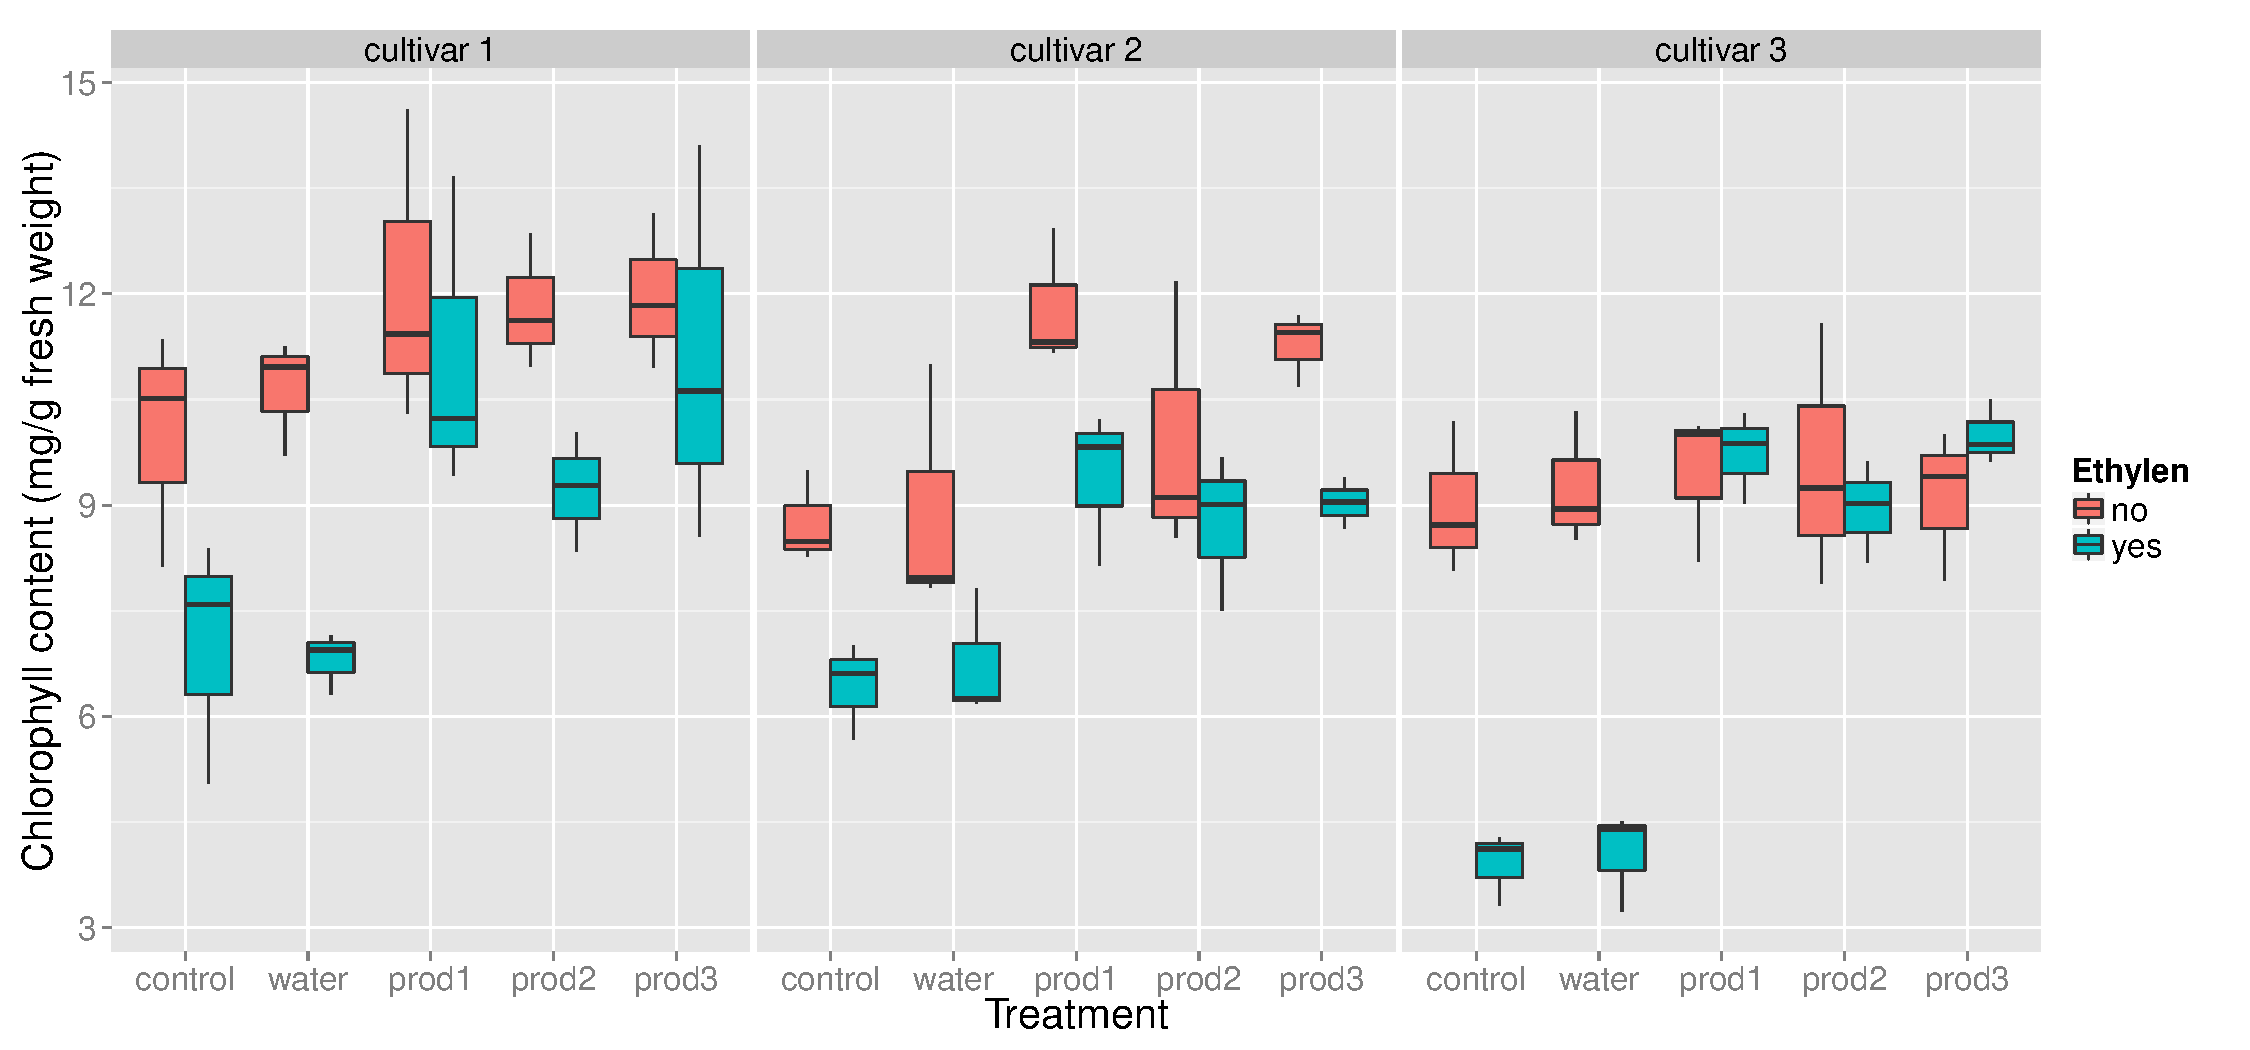
\includegraphics[width=\maxwidth]{figure/chunk62} \caption[Boxplots of the chlorophyll content after eight days based on each ethylene-by-treatment-by-cultivar combination]{Boxplots of the chlorophyll content after eight days based on each ethylene-by-treatment-by-cultivar combination.\label{fig:chunk62}}
\end{figure}


\end{knitrout}


% latex table generated in R 3.0.2 by xtable 1.7-1 package
% Mon Mar 24 09:14:20 2014
\begin{table}[ht]
\centering
\begin{tabular}{lrrrrr}
  \hline
 & Df & Sum Sq & Mean Sq & F value & Pr($>$F) \\ 
  \hline
Cult & 2 & 53.22 & 26.61 & 16.00 & 0.0000 \\ 
  Eth & 1 & 98.85 & 98.85 & 59.43 & 0.0000 \\ 
  Treatment & 4 & 156.05 & 39.01 & 23.46 & 0.0000 \\ 
  Cult:Eth & 2 & 0.37 & 0.19 & 0.11 & 0.8938 \\ 
  Cult:Treatment & 8 & 3.05 & 0.38 & 0.23 & 0.9840 \\ 
  Eth:Treatment & 4 & 35.65 & 8.91 & 5.36 & 0.0009 \\ 
  Cult:Eth:Treatment & 8 & 28.73 & 3.59 & 2.16 & 0.0436 \\ 
  Residuals & 60 & 99.80 & 1.66 &  &  \\ 
   \hline
\end{tabular}
\caption{Three-way ANOVA table of the ethylene blocking data set.} 
\end{table}


The following one-way contrast matrices are used to analyse the ethylene-by-treatment interaction. 
\begin{knitrout}
\definecolor{shadecolor}{rgb}{0.969, 0.969, 0.969}\color{fgcolor}\begin{kframe}
\begin{alltt}
\hlcom{#definition of appropriate contrasts}
\hlcom{#1. contrast for the different ethylen treatments}
\hlstd{ContrMat_Ethylen} \hlkwb{<-} \hlkwd{matrix}\hlstd{(}\hlkwd{c}\hlstd{(}\hlnum{1}\hlstd{,} \hlopt{-}\hlnum{1}\hlstd{),} \hlkwc{nrow}\hlstd{=}\hlnum{1}\hlstd{,} \hlkwc{byrow}\hlstd{=}\hlnum{FALSE}\hlstd{)}
\hlcom{#2. contrasts for the Treatment factor }
\hlstd{ContrMat_Treatment} \hlkwb{<-} \hlkwd{matrix}\hlstd{(}\hlkwd{c}\hlstd{(}\hlnum{1}\hlopt{/}\hlnum{2}\hlstd{,} \hlnum{1}\hlopt{/}\hlnum{2}\hlstd{,}\hlopt{-}\hlnum{1}\hlopt{/}\hlnum{3}\hlstd{,}\hlopt{-}\hlnum{1}\hlopt{/}\hlnum{3}\hlstd{,}\hlopt{-}\hlnum{1}\hlopt{/}\hlnum{3}\hlstd{,}
                                 \hlnum{0}\hlstd{,}   \hlnum{0}\hlstd{,}   \hlnum{1}\hlstd{,}  \hlopt{-}\hlnum{1}\hlstd{,}   \hlnum{0}\hlstd{,}
                                 \hlnum{0}\hlstd{,}   \hlnum{0}\hlstd{,}   \hlnum{1}\hlstd{,}   \hlnum{0}\hlstd{,}  \hlopt{-}\hlnum{1}\hlstd{,}
                                 \hlnum{0}\hlstd{,}   \hlnum{0}\hlstd{,}   \hlnum{0}\hlstd{,}   \hlnum{1}\hlstd{,}  \hlopt{-}\hlnum{1}\hlstd{),}
                             \hlkwc{nrow}\hlstd{=}\hlnum{4}\hlstd{,} \hlkwc{byrow}\hlstd{=}\hlnum{TRUE}\hlstd{)}
\end{alltt}
\end{kframe}
\end{knitrout}

Since there is also a significant cultivar-by-treatment-by-ethylene interaction, the interaction contrast matrix has to be defined manually by using the Kronecker product. 
\begin{knitrout}
\definecolor{shadecolor}{rgb}{0.969, 0.969, 0.969}\color{fgcolor}\begin{kframe}
\begin{alltt}
\hlstd{ContrMat_Cult} \hlkwb{<-} \hlkwd{matrix}\hlstd{(}\hlkwd{c}\hlstd{(}\hlnum{1}\hlopt{/}\hlnum{3}\hlstd{,}\hlnum{1}\hlopt{/}\hlnum{3}\hlstd{,}\hlnum{1}\hlopt{/}\hlnum{3}\hlstd{),}
                        \hlkwc{nrow}\hlstd{=}\hlnum{1}\hlstd{)}
\hlcom{#interaction contrast matrix}
\hlstd{InteractionContrasts}\hlkwb{<-} \hlkwd{kronecker}\hlstd{(ContrMat_Cult,}
                       \hlkwd{kronecker}\hlstd{(ContrMat_Treatment, ContrMat_Ethylen))}
\hlcom{#fitting the appropriate cell means model}
\hlstd{ethylen}\hlopt{$}\hlstd{CultTreatEth} \hlkwb{<-} \hlkwd{with}\hlstd{(ethylen, Cult}\hlopt{:}\hlstd{Treatment}\hlopt{:}\hlstd{Eth)}
\hlstd{CMM} \hlkwb{<-} \hlkwd{lm}\hlstd{(Chloro8} \hlopt{~} \hlstd{CultTreatEth}\hlopt{-}\hlnum{1}\hlstd{,} \hlkwc{data}\hlstd{=ethylen)}
\hlkwd{library}\hlstd{(multcomp)}
\hlstd{MultTest} \hlkwb{<-} \hlkwd{glht}\hlstd{(CMM,} \hlkwc{linfct}\hlstd{=}\hlkwd{mcp}\hlstd{(}\hlkwc{CultTreatEth}\hlstd{=InteractionContrasts))}
\hlkwd{summary}\hlstd{(MultTest)}
\hlkwd{confint}\hlstd{(MultTest)}
\end{alltt}
\end{kframe}
\end{knitrout}


For illustrative purposes we additionally demonstrate the analysis of the cultivar-by-treatment-by ethylene interaction. Therefore we consider that all pairwise conparisons of the cultivars are of interest. 
\begin{knitrout}
\definecolor{shadecolor}{rgb}{0.969, 0.969, 0.969}\color{fgcolor}\begin{kframe}
\begin{alltt}
\hlstd{CultMatrix} \hlkwb{<-} \hlkwd{matrix}\hlstd{(}\hlkwd{c}\hlstd{(}\hlnum{1}\hlstd{,} \hlopt{-}\hlnum{1}\hlstd{,} \hlnum{0}\hlstd{,}
                       \hlnum{1}\hlstd{,}  \hlnum{0}\hlstd{,}\hlopt{-}\hlnum{1}\hlstd{,}
                       \hlnum{0}\hlstd{,}  \hlnum{1}\hlstd{,}\hlopt{-}\hlnum{1}\hlstd{),} \hlkwc{nrow}\hlstd{=}\hlnum{3}\hlstd{,} \hlkwc{byrow}\hlstd{=}\hlnum{TRUE}\hlstd{)}
\hlstd{InteractionContrasts}\hlkwb{<-} \hlkwd{kronecker}\hlstd{(CultMatrix,}
                       \hlkwd{kronecker}\hlstd{(ContrMat_Treatment, ContrMat_Ethylen))}
\hlstd{MultTest} \hlkwb{<-} \hlkwd{glht}\hlstd{(CMM,} \hlkwc{linfct}\hlstd{=}\hlkwd{mcp}\hlstd{(}\hlkwc{CultTreatEth}\hlstd{=InteractionContrasts))}
\hlkwd{summary}\hlstd{(MultTest)}
\hlkwd{confint}\hlstd{(MultTest)}
\end{alltt}
\end{kframe}
\end{knitrout}


% latex table generated in R 3.0.2 by xtable 1.7-1 package
% Mon Mar 24 09:14:23 2014
\begin{table}[ht]
\centering
{\scriptsize
\begin{tabular}{rrrrr}
  \hline
 & Estimate & Std.Error & t value & Pr($>$$|$t$|$) \\ 
  \hline
Ethylene (control - Product)Cult1-Cult2 & 1.62 & 1.36 & 1.19 & 0.86 \\ 
  Ethylene (Prod1 - Prod2)Cult1-Cult2 & -2.78 & 2.11 & -1.32 & 0.79 \\ 
  Ethylene (Prod1 - Prod3)Cult1-Cult2 & -0.04 & 2.11 & -0.02 & 1.00 \\ 
  Ethylene (Prod2 - Prod3)Cult1-Cult2 & 2.75 & 2.11 & 1.30 & 0.80 \\ 
  Ethylene (control - Product)Cult1-Cult3 & -3.42 & 1.36 & -2.51 & 0.13 \\ 
  Ethylene (Prod1 - Prod2)Cult1-Cult3 & -0.66 & 2.11 & -0.31 & 1.00 \\ 
  Ethylene (Prod1 - Prod3)Cult1-Cult3 & -0.45 & 2.11 & -0.22 & 1.00 \\ 
  Ethylene (Prod2 - Prod3)Cult1-Cult3 & 0.21 & 2.11 & 0.10 & 1.00 \\ 
  Ethylene (control - Product)Cult2-Cult3 & -5.04 & 1.36 & -3.71 & 0.00 \\ 
  Ethylene (Prod1 - Prod2)Cult2-Cult3 & 2.12 & 2.11 & 1.01 & 0.93 \\ 
  Ethylene (Prod1 - Prod3)Cult2-Cult3 & -0.42 & 2.11 & -0.20 & 1.00 \\ 
  Ethylene (Prod2 - Prod3)Cult2-Cult3 & -2.54 & 2.11 & -1.20 & 0.86 \\ 
   \hline
\end{tabular}
}
\caption{Results for the three-way interaction analysis of the ethylene blocking data set. Estimate denote the estimate for the comparison of interest, the adjusted P-value, Lower and Upper the lower and upper bound of the two-sided 0.95 simultaneous confidence interval.} 
\end{table}



\newpage

\section{Water deficiency data set}
This data set was part of an experiment conducted at the Woody Plant and Propagation Physiology Section in the Institute of Horticultural Production Systems at the Leibniz Universität Hannover in 2013. The goal of the experiment was to investigate a potential differing response among nine varieties of starch potato (\emph{Solanum tuberosum}) on water deficiency stress.  The following nine varieties of starch potato were selected for cultivation: A, B, C, D, E, F, G, H and I. Each variety was cultivated under four different water conditions: standard control medium, 0.1M, 0.2M and 0.3M sorbitol medium. An increasing sorbitol concentration was used to induce an increasing water deficiency stress on the plants. For each treatment by variety combination 6 replicates were investigated. The trial was planned in a completely cross-classified treatment structure, in a completely randomized design. A total number of 13 objects were discarded from the analysis because of infection diseases. For each experimental unit the fresh weight of the shoot was measured. To achieve approximately equal variances over the factor levels of the response variable a log transformation was performed.


\begin{knitrout}
\definecolor{shadecolor}{rgb}{0.969, 0.969, 0.969}\color{fgcolor}\begin{kframe}
\begin{alltt}
\hlkwd{library}\hlstd{(statint)}
\hlkwd{data}\hlstd{(potato)}
\hlkwd{str}\hlstd{(potato)}
\hlstd{potato}\hlopt{$}\hlstd{treatment} \hlkwb{<-} \hlkwd{factor}\hlstd{(potato}\hlopt{$}\hlstd{treatment,}
                           \hlkwc{levels}\hlstd{=}\hlkwd{c}\hlstd{(}\hlstr{"control"}\hlstd{,}\hlstr{"0.1"}\hlstd{,}\hlstr{"0.2"}\hlstd{,}\hlstr{"0.3"}\hlstd{))}
\end{alltt}
\end{kframe}
\end{knitrout}

\begin{knitrout}
\definecolor{shadecolor}{rgb}{0.969, 0.969, 0.969}\color{fgcolor}\begin{figure}[]

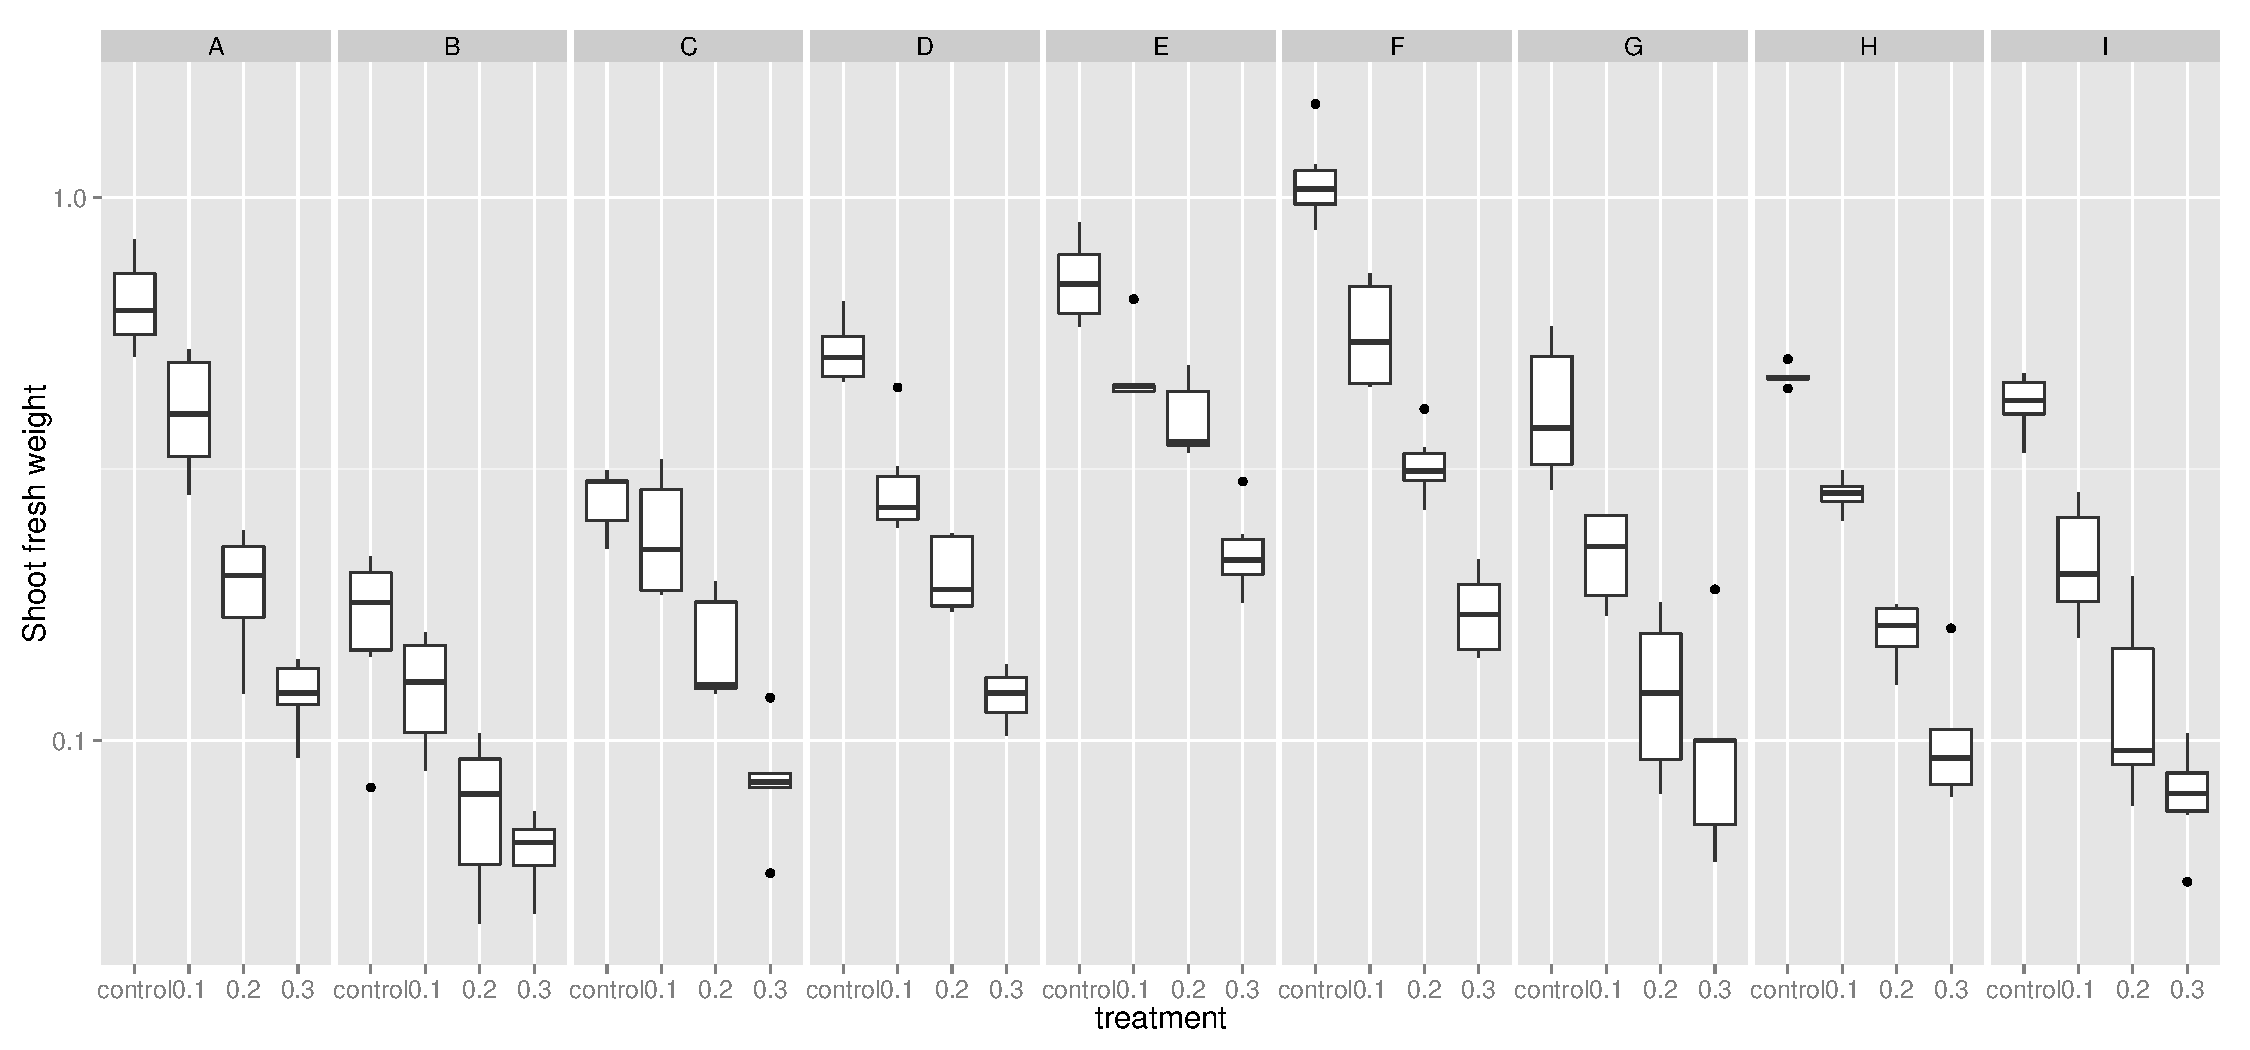
\includegraphics[width=\maxwidth]{figure/chunk41} \caption[Boxplots of the shoot fresh weight based on each variety-by-stress combination]{Boxplots of the shoot fresh weight based on each variety-by-stress combination.\label{fig:chunk41}}
\end{figure}


\end{knitrout}


The researcher was interested in selecting those varieties with a different response on water deficiency in contrast to the general water deficiency response. Additionally, interest was in determining on which level of water deficiency stress those potential deviations occur.  
% latex table generated in R 3.0.2 by xtable 1.7-1 package
% Mon Mar 24 09:14:24 2014
\begin{table}[ht]
\centering
\begin{tabular}{lrrrrr}
  \hline
 & Df & Sum Sq & Mean Sq & F value & Pr($>$F) \\ 
  \hline
treatment & 3 & 57.02 & 19.01 & 356.98 & 0.0000 \\ 
  genotype & 8 & 40.96 & 5.12 & 96.16 & 0.0000 \\ 
  treatment:genotype & 24 & 2.93 & 0.12 & 2.30 & 0.0012 \\ 
  Residuals & 167 & 8.89 & 0.05 &  &  \\ 
   \hline
\end{tabular}
\caption{Two-way ANOVA table of the water defciency data set} 
\end{table}



\begin{knitrout}
\definecolor{shadecolor}{rgb}{0.969, 0.969, 0.969}\color{fgcolor}\begin{kframe}
\begin{alltt}
\hlstd{InteractionContrasts} \hlkwb{<-} \hlkwd{iacontrast}\hlstd{(}\hlkwc{fa}\hlstd{=potato}\hlopt{$}\hlstd{treatment,}
                                   \hlkwc{fb}\hlstd{=potato}\hlopt{$}\hlstd{genotype,}
                                    \hlkwc{typea}\hlstd{=}\hlstr{"Dunnett"}\hlstd{,} \hlkwc{typeb}\hlstd{=}\hlstr{"GrandMean"}\hlstd{)}
\hlstd{potato}\hlopt{$}\hlstd{GenTreat} \hlkwb{<-} \hlstd{InteractionContrasts}\hlopt{$}\hlstd{fab}
\hlstd{CellMeansModel} \hlkwb{<-} \hlkwd{lm}\hlstd{(}\hlkwd{log}\hlstd{(shoot)} \hlopt{~} \hlstd{GenTreat}\hlopt{-}\hlnum{1}\hlstd{,} \hlkwc{data}\hlstd{=potato)}
\hlcom{#conducting user defined multiple comparisons}
\hlstd{MultTest} \hlkwb{<-} \hlkwd{glht}\hlstd{(}\hlkwc{model}\hlstd{=CellMeansModel,}
                 \hlkwc{linfct} \hlstd{=} \hlkwd{mcp}\hlstd{(}\hlkwc{GenTreat}\hlstd{=InteractionContrasts}\hlopt{$}\hlstd{cmab))}
\hlkwd{summary}\hlstd{(MultTest)}\hlcom{#calculating adjusted p-values}
\hlstd{ConfInt} \hlkwb{<-} \hlkwd{confint}\hlstd{(MultTest)}\hlcom{#calculating simultaneous confidence intervals}
\end{alltt}
\end{kframe}
\end{knitrout}


% latex table generated in R 3.0.2 by xtable 1.7-1 package
% Mon Mar 24 09:14:40 2014
\begin{table}[ht]
\centering
{\small
\begin{tabular}{rrrrr}
  \hline
 & Estimate & Std.Error & t value & Pr($>$$|$t$|$) \\ 
  \hline
((0.1 - control):A) - ((0.1 - control):B,C,D,E,F,G,H,I) & 0.00 & 0.13 & 0.03 & 1.00 \\ 
  ((0.1 - control):B) - ((0.1 - control):A,C,D,E,F,G,H,I) & 0.21 & 0.13 & 1.69 & 0.87 \\ 
  ((0.1 - control):C) - ((0.1 - control):A,B,D,E,F,G,H,I) & 0.32 & 0.14 & 2.36 & 0.36 \\ 
  ((0.1 - control):D) - ((0.1 - control):A,B,C,E,F,G,H,I) & -0.09 & 0.13 & -0.75 & 1.00 \\ 
  ((0.1 - control):E) - ((0.1 - control):A,B,C,D,F,G,H,I) & 0.09 & 0.13 & 0.72 & 1.00 \\ 
  ((0.1 - control):F) - ((0.1 - control):A,B,C,D,E,G,H,I) & -0.18 & 0.13 & -1.41 & 0.97 \\ 
  ((0.1 - control):G) - ((0.1 - control):A,B,C,D,E,F,H,I) & -0.13 & 0.13 & -1.05 & 1.00 \\ 
  ((0.1 - control):H) - ((0.1 - control):A,B,C,D,E,F,G,I) & -0.02 & 0.14 & -0.18 & 1.00 \\ 
  ((0.1 - control):I) - ((0.1 - control):A,B,C,D,E,F,G,H) & -0.21 & 0.13 & -1.64 & 0.90 \\ 
  ((0.2 - control):A) - ((0.2 - control):B,C,D,E,F,G,H,I) & -0.22 & 0.13 & -1.75 & 0.84 \\ 
  ((0.2 - control):B) - ((0.2 - control):A,C,D,E,F,G,H,I) & 0.22 & 0.13 & 1.73 & 0.85 \\ 
  ((0.2 - control):C) - ((0.2 - control):A,B,D,E,F,G,H,I) & 0.36 & 0.14 & 2.66 & 0.19 \\ 
  ((0.2 - control):D) - ((0.2 - control):A,B,C,E,F,G,H,I) & 0.05 & 0.13 & 0.38 & 1.00 \\ 
  ((0.2 - control):E) - ((0.2 - control):A,B,C,D,F,G,H,I) & 0.40 & 0.13 & 3.21 & 0.04 \\ 
  ((0.2 - control):F) - ((0.2 - control):A,B,C,D,E,G,H,I) & -0.21 & 0.13 & -1.66 & 0.89 \\ 
  ((0.2 - control):G) - ((0.2 - control):A,B,C,D,E,F,H,I) & -0.20 & 0.13 & -1.60 & 0.92 \\ 
  ((0.2 - control):H) - ((0.2 - control):A,B,C,D,E,F,G,I) & -0.10 & 0.14 & -0.70 & 1.00 \\ 
  ((0.2 - control):I) - ((0.2 - control):A,B,C,D,E,F,G,H) & -0.31 & 0.13 & -2.43 & 0.31 \\ 
  ((0.3 - control):A) - ((0.3 - control):B,C,D,E,F,G,H,I) & -0.23 & 0.13 & -1.82 & 0.79 \\ 
  ((0.3 - control):B) - ((0.3 - control):A,C,D,E,F,G,H,I) & 0.49 & 0.14 & 3.50 & 0.02 \\ 
  ((0.3 - control):C) - ((0.3 - control):A,B,D,E,F,G,H,I) & 0.24 & 0.14 & 1.72 & 0.85 \\ 
  ((0.3 - control):D) - ((0.3 - control):A,B,C,E,F,G,H,I) & -0.03 & 0.13 & -0.22 & 1.00 \\ 
  ((0.3 - control):E) - ((0.3 - control):A,B,C,D,F,G,H,I) & 0.28 & 0.13 & 2.22 & 0.47 \\ 
  ((0.3 - control):F) - ((0.3 - control):A,B,C,D,E,G,H,I) & -0.40 & 0.13 & -3.18 & 0.04 \\ 
  ((0.3 - control):G) - ((0.3 - control):A,B,C,D,E,F,H,I) & -0.00 & 0.13 & -0.00 & 1.00 \\ 
  ((0.3 - control):H) - ((0.3 - control):A,B,C,D,E,F,G,I) & -0.11 & 0.14 & -0.78 & 1.00 \\ 
  ((0.3 - control):I) - ((0.3 - control):A,B,C,D,E,F,G,H) & -0.24 & 0.13 & -1.88 & 0.75 \\ 
   \hline
\end{tabular}
}
\caption{Results for the interaction analysis of the Water deficiency data set. Estimate denote the estimate for the comparison of interest, the adjusted P-value, Lower and Upper the lower and upper bound of the two-sided 0.95 simultaneous confidence interval} 
\end{table}





\newpage

\section{Oats Field Trial}
In this section the analysis of statistical interaction in a split-plot field trial is demonstrated. 
The underlying methodoly is roughly described in \cite{Kitsche.2014}.
Therefore, the \verb@oats@ dataset from the R add-on package \verb@MASS@ is used \citep{Venables2002}. In this trial the yield of three different varieties of oats was investigated unter four levels of manurial treatment. For a detailed description we refer to the \verb@MASS@ package documentation of the data set. 


\begin{knitrout}
\definecolor{shadecolor}{rgb}{0.969, 0.969, 0.969}\color{fgcolor}\begin{figure}[]

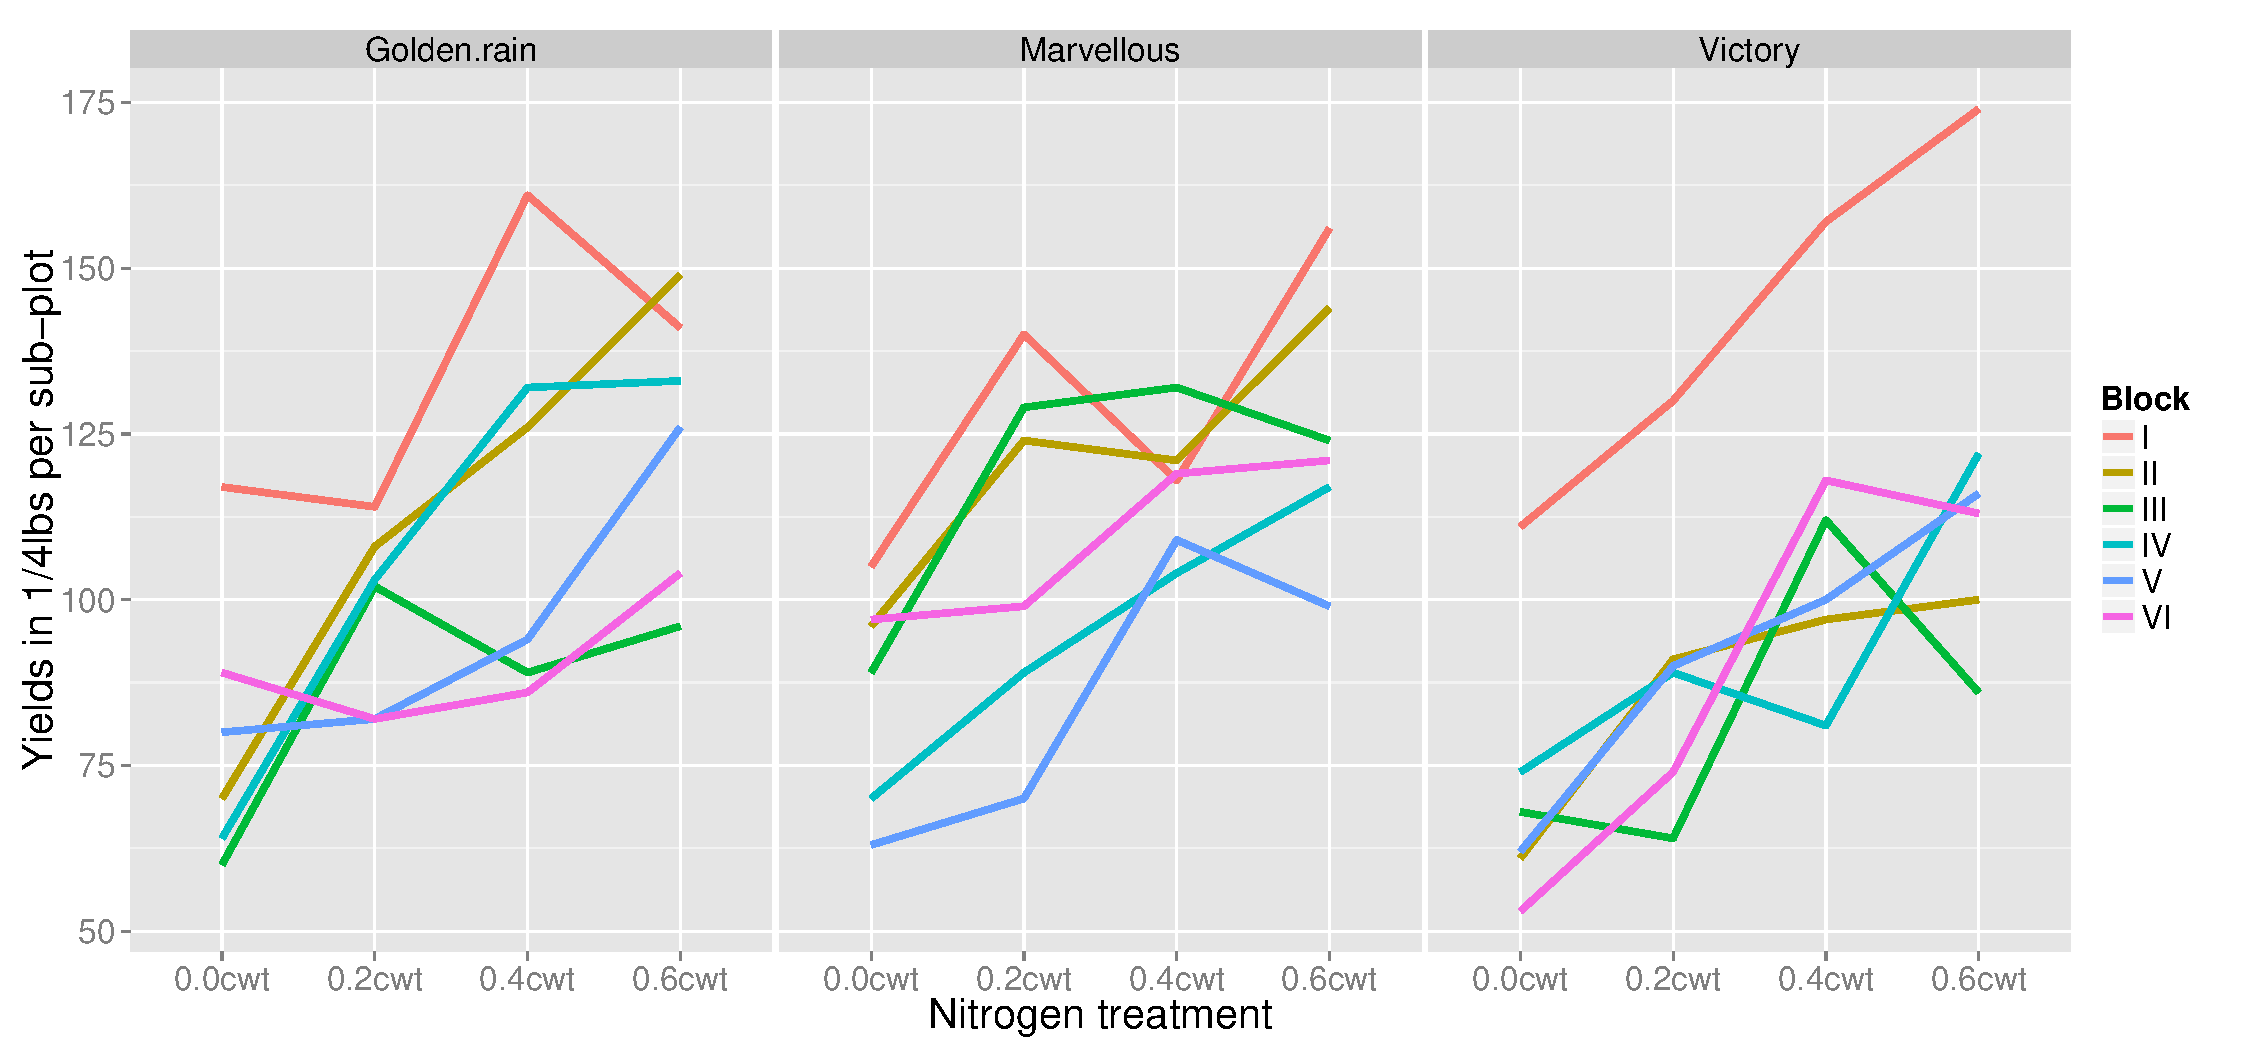
\includegraphics[width=\maxwidth]{figure/chunk51_} \caption[Interaction plot of the oats field trial]{Interaction plot of the oats field trial.\label{fig:chunk51,}}
\end{figure}


\end{knitrout}


\begin{knitrout}
\definecolor{shadecolor}{rgb}{0.969, 0.969, 0.969}\color{fgcolor}\begin{kframe}
\begin{alltt}
\hlkwd{library}\hlstd{(nlme)}
\hlstd{fit} \hlkwb{<-} \hlkwd{lme}\hlstd{(Y} \hlopt{~} \hlstd{N} \hlopt{+} \hlstd{V} \hlopt{+} \hlstd{N}\hlopt{:}\hlstd{V,} \hlkwc{data} \hlstd{= oats,} \hlkwc{random} \hlstd{=} \hlopt{~}\hlnum{1} \hlopt{|} \hlstd{B}\hlopt{/}\hlstd{V)}
\hlkwd{anova}\hlstd{(fit)}
\end{alltt}
\end{kframe}
\end{knitrout}



% latex table generated in R 3.0.2 by xtable 1.7-1 package
% Mon Mar 24 09:14:40 2014
\begin{table}[ht]
\centering
\begin{tabular}{rrrrr}
  \hline
 & numDF & denDF & F-value & p-value \\ 
  \hline
(Intercept) &   1 & 45.00 & 245.14 & 0.00 \\ 
  N &   3 & 45.00 & 37.69 & 0.00 \\ 
  V &   2 & 10.00 & 1.49 & 0.27 \\ 
  N:V &   6 & 45.00 & 0.30 & 0.93 \\ 
   \hline
\end{tabular}
\caption{ANOVA of the split-plot oats field trial.} 
\end{table}



Although there is no evidence for an interaction in this trial, we further assume that interest is in the anylsis of the nitrogen-by-variety interaction for illustrative purposes.  
\begin{knitrout}
\definecolor{shadecolor}{rgb}{0.969, 0.969, 0.969}\color{fgcolor}\begin{kframe}
\begin{alltt}
\hlstd{InteractionContrasts} \hlkwb{<-} \hlkwd{iacontrast}\hlstd{(}\hlkwc{fa}\hlstd{=oats}\hlopt{$}\hlstd{N,} \hlkwc{fb}\hlstd{=oats}\hlopt{$}\hlstd{V,}
                                   \hlkwc{typea} \hlstd{=} \hlstr{"Tukey"}\hlstd{,} \hlkwc{typeb} \hlstd{=} \hlstr{"Tukey"}\hlstd{,}
                                   \hlkwc{abbrevnames}\hlstd{=}\hlkwd{list}\hlstd{(}\hlstr{"minlength"}\hlstd{=}\hlnum{4}\hlstd{))}
\hlstd{oats}\hlopt{$}\hlstd{NV} \hlkwb{<-} \hlstd{InteractionContrasts}\hlopt{$}\hlstd{fab}
\hlcom{#fitting the cell means model}
\hlstd{CMM} \hlkwb{<-} \hlkwd{lme}\hlstd{(Y} \hlopt{~} \hlstd{NV,} \hlkwc{data}\hlstd{=oats,} \hlkwc{random}\hlstd{=}\hlopt{~}\hlnum{1}\hlopt{|}\hlstd{B}\hlopt{/}\hlstd{V)}
\hlkwd{anova}\hlstd{(CMM)}
\hlcom{# In principle, there may be more appropriate denominator degrees }
\hlcom{# of freedom here. For consistency with ANOVA we select 43}
\hlstd{MultTest} \hlkwb{<-} \hlkwd{glht}\hlstd{(CMM,} \hlkwd{mcp}\hlstd{(}\hlkwc{NV} \hlstd{= InteractionContrasts}\hlopt{$}\hlstd{cmab),} \hlkwc{df}\hlstd{=}\hlnum{43}\hlstd{)}
\hlkwd{summary}\hlstd{(MultTest)}
\hlkwd{confint}\hlstd{(MultTest)}
\end{alltt}
\end{kframe}
\end{knitrout}



\newpage
\bibliographystyle{apalike}
\bibliography{References_HortInt}
\end{document}
